% Options for packages loaded elsewhere
\PassOptionsToPackage{unicode}{hyperref}
\PassOptionsToPackage{hyphens}{url}
%
\documentclass[
  english,
  man,floatsintext]{apa6}
\usepackage{amsmath,amssymb}
\usepackage{lmodern}
\usepackage{ifxetex,ifluatex}
\ifnum 0\ifxetex 1\fi\ifluatex 1\fi=0 % if pdftex
  \usepackage[T1]{fontenc}
  \usepackage[utf8]{inputenc}
  \usepackage{textcomp} % provide euro and other symbols
\else % if luatex or xetex
  \usepackage{unicode-math}
  \defaultfontfeatures{Scale=MatchLowercase}
  \defaultfontfeatures[\rmfamily]{Ligatures=TeX,Scale=1}
\fi
% Use upquote if available, for straight quotes in verbatim environments
\IfFileExists{upquote.sty}{\usepackage{upquote}}{}
\IfFileExists{microtype.sty}{% use microtype if available
  \usepackage[]{microtype}
  \UseMicrotypeSet[protrusion]{basicmath} % disable protrusion for tt fonts
}{}
\makeatletter
\@ifundefined{KOMAClassName}{% if non-KOMA class
  \IfFileExists{parskip.sty}{%
    \usepackage{parskip}
  }{% else
    \setlength{\parindent}{0pt}
    \setlength{\parskip}{6pt plus 2pt minus 1pt}}
}{% if KOMA class
  \KOMAoptions{parskip=half}}
\makeatother
\usepackage{xcolor}
\IfFileExists{xurl.sty}{\usepackage{xurl}}{} % add URL line breaks if available
\IfFileExists{bookmark.sty}{\usepackage{bookmark}}{\usepackage{hyperref}}
\hypersetup{
  pdftitle={Preferring Politeness: Young children's implicit comprehension of linguistic politeness},
  pdfauthor={Hannah E. Marshall1, Rondeline M. Williams1, \& Michael C. Frank1},
  pdflang={en-EN},
  pdfkeywords={politeness, language acquisition, pragmatic development, online experiment},
  hidelinks,
  pdfcreator={LaTeX via pandoc}}
\urlstyle{same} % disable monospaced font for URLs
\usepackage{graphicx}
\makeatletter
\def\maxwidth{\ifdim\Gin@nat@width>\linewidth\linewidth\else\Gin@nat@width\fi}
\def\maxheight{\ifdim\Gin@nat@height>\textheight\textheight\else\Gin@nat@height\fi}
\makeatother
% Scale images if necessary, so that they will not overflow the page
% margins by default, and it is still possible to overwrite the defaults
% using explicit options in \includegraphics[width, height, ...]{}
\setkeys{Gin}{width=\maxwidth,height=\maxheight,keepaspectratio}
% Set default figure placement to htbp
\makeatletter
\def\fps@figure{htbp}
\makeatother
\setlength{\emergencystretch}{3em} % prevent overfull lines
\providecommand{\tightlist}{%
  \setlength{\itemsep}{0pt}\setlength{\parskip}{0pt}}
\setcounter{secnumdepth}{-\maxdimen} % remove section numbering
% Make \paragraph and \subparagraph free-standing
\ifx\paragraph\undefined\else
  \let\oldparagraph\paragraph
  \renewcommand{\paragraph}[1]{\oldparagraph{#1}\mbox{}}
\fi
\ifx\subparagraph\undefined\else
  \let\oldsubparagraph\subparagraph
  \renewcommand{\subparagraph}[1]{\oldsubparagraph{#1}\mbox{}}
\fi
% Manuscript styling
\usepackage{upgreek}
\captionsetup{font=singlespacing,justification=justified}

% Table formatting
\usepackage{longtable}
\usepackage{lscape}
% \usepackage[counterclockwise]{rotating}   % Landscape page setup for large tables
\usepackage{multirow}		% Table styling
\usepackage{tabularx}		% Control Column width
\usepackage[flushleft]{threeparttable}	% Allows for three part tables with a specified notes section
\usepackage{threeparttablex}            % Lets threeparttable work with longtable

% Create new environments so endfloat can handle them
% \newenvironment{ltable}
%   {\begin{landscape}\begin{center}\begin{threeparttable}}
%   {\end{threeparttable}\end{center}\end{landscape}}
\newenvironment{lltable}{\begin{landscape}\begin{center}\begin{ThreePartTable}}{\end{ThreePartTable}\end{center}\end{landscape}}

% Enables adjusting longtable caption width to table width
% Solution found at http://golatex.de/longtable-mit-caption-so-breit-wie-die-tabelle-t15767.html
\makeatletter
\newcommand\LastLTentrywidth{1em}
\newlength\longtablewidth
\setlength{\longtablewidth}{1in}
\newcommand{\getlongtablewidth}{\begingroup \ifcsname LT@\roman{LT@tables}\endcsname \global\longtablewidth=0pt \renewcommand{\LT@entry}[2]{\global\advance\longtablewidth by ##2\relax\gdef\LastLTentrywidth{##2}}\@nameuse{LT@\roman{LT@tables}} \fi \endgroup}

% \setlength{\parindent}{0.5in}
% \setlength{\parskip}{0pt plus 0pt minus 0pt}

% \usepackage{etoolbox}
\makeatletter
\patchcmd{\HyOrg@maketitle}
  {\section{\normalfont\normalsize\abstractname}}
  {\section*{\normalfont\normalsize\abstractname}}
  {}{\typeout{Failed to patch abstract.}}
\patchcmd{\HyOrg@maketitle}
  {\section{\protect\normalfont{\@title}}}
  {\section*{\protect\normalfont{\@title}}}
  {}{\typeout{Failed to patch title.}}
\makeatother
\shorttitle{Preferring Politeness}
\keywords{politeness, language acquisition, pragmatic development, online experiment\newline\indent Word count: 4,990}
\usepackage{lineno}

\linenumbers
\usepackage{csquotes}
\ifxetex
  % Load polyglossia as late as possible: uses bidi with RTL langages (e.g. Hebrew, Arabic)
  \usepackage{polyglossia}
  \setmainlanguage[]{english}
\else
  \usepackage[main=english]{babel}
% get rid of language-specific shorthands (see #6817):
\let\LanguageShortHands\languageshorthands
\def\languageshorthands#1{}
\fi
\ifluatex
  \usepackage{selnolig}  % disable illegal ligatures
\fi
\newlength{\cslhangindent}
\setlength{\cslhangindent}{1.5em}
\newlength{\csllabelwidth}
\setlength{\csllabelwidth}{3em}
\newenvironment{CSLReferences}[2] % #1 hanging-ident, #2 entry spacing
 {% don't indent paragraphs
  \setlength{\parindent}{0pt}
  % turn on hanging indent if param 1 is 1
  \ifodd #1 \everypar{\setlength{\hangindent}{\cslhangindent}}\ignorespaces\fi
  % set entry spacing
  \ifnum #2 > 0
  \setlength{\parskip}{#2\baselineskip}
  \fi
 }%
 {}
\usepackage{calc}
\newcommand{\CSLBlock}[1]{#1\hfill\break}
\newcommand{\CSLLeftMargin}[1]{\parbox[t]{\csllabelwidth}{#1}}
\newcommand{\CSLRightInline}[1]{\parbox[t]{\linewidth - \csllabelwidth}{#1}\break}
\newcommand{\CSLIndent}[1]{\hspace{\cslhangindent}#1}

\title{Preferring Politeness: Young children's implicit comprehension of linguistic politeness}
\author{Hannah E. Marshall\textsuperscript{1}, Rondeline M. Williams\textsuperscript{1}, \& Michael C. Frank\textsuperscript{1}}
\date{}


\authornote{

I would like to thank Professor Michael C. Frank for his leadership, encouragement, and support throughout this project. Thank you also to Rondeline M. Williams, who has dedicated so much time and energy into supporting me as a researcher and friend. I would also like to thank the members of the Language and Cognition Lab at Stanford University, who offered invaluable feedback on the theory, methods, and interpretation contained in this thesis. Finally, I would like to thank Professor Jeffrey J. Wine, the late Professor Lee Ross, and Cai Guo for their expertise, guidance, and support throughout my time in the Psychology Senior Honors Program. This research was made possible in part by the Psych-Summer Research Program and was supported by a stipend from the Vice Provost for Undergraduate Education at Stanford University. The authors declare no conflict of interest.

Correspondence concerning this article should be addressed to Hannah E. Marshall. E-mail: \href{mailto:hannah21@stanford.edu}{\nolinkurl{hannah21@stanford.edu}}

}

\affiliation{\vspace{0.5cm}\textsuperscript{1} Stanford University}

\abstract{
Adults routinely demonstrate social sensitivity by utilizing polite speech. But when do children begin to comprehend linguistic politeness? Existing literature indicates that basic comprehension of polite speech presents early in development; however, previous studies have not observed reliable preference for a polite speaker in children younger than 4 years, potentially due to experimental task demands. This project uses a less challenging paradigm (adapted from similar shape-preference paradigms, i.e., Hamlin, Wynn, \& Bloom, 2007; Thomas \& Sarnecka, 2019) to investigate the age of polite language acquisition. Our data showed that 2-year-old and 4-year-old children indicate preference for a polite speaker, whereas 3-year-old children indicate preference for an impolite speaker, suggesting either that our data underestimate the preference of 3-year-old children or that preference for a polite speaker--and perhaps comprehension and acquisition of linguistic politeness more broadly--does not develop as a smooth trend across development. In addition to informing our understanding of children's sociolinguistic development, this study demonstrates the effectiveness of a simpler paradigm for future studies of linguistic politeness in young children.
}



\begin{document}
\maketitle

To engage in successful social interactions, an individual must demonstrate social sensitivity; the same individual must assess the social sensitivity of others to determine the desirability of their social partners. The capacity to evaluate individuals on the basis of their social interactions is universal and unlearned (Haidt \& Joseph, 2004; Hamlin, Wynn, \& Bloom, 2007; Hauser, 2006; Pinker, 2003). Even preverbal infants develop social preferences based on individuals' behavior toward others (Hamlin, Wynn, \& Bloom, 2007). Through development, humans learn to routinely demonstrate and assess social sensitivity by employing and interpreting linguistic politeness in speech.

Linguistic politeness can be defined as a set of social behaviors, expressed verbally, which maintain, enhance, or challenge interpersonal relations (Vergis \& Pell, 2020). It is a form of social etiquette, which regulates the choice of communicative forms, structures, and set phrases a person uses (Ryabova, 2015). Being polite is considered a part of adult pragmatic competence. According to Lakoff's (1973) Politeness Principles, the rules of politeness include \emph{Distance} (do not impose), \emph{Deference} (give options), and \emph{Camaraderie} (make the addressee feel good).

Grice (1975) asserts that, when conversing, rational speakers strive to obey four maxims: \emph{Quality} (speak truthfully), \emph{Quantity} (speak succinctly), \emph{Relation} (speak relevantly), and \emph{Manner} (speak clearly). These maxims describe the basis of human communication. When speaking politely, however, individuals typically do not behave rationally in accordance with Gricean Maxims: in fact, polite speech violates theories of effective communication by typically being both inefficient, indirect, and under-informative (Yoon, Tessler, Goodman, \& Frank, 2020). Then why speak politely?

Yoon et al. (2020) propose a utility-theoretic solution to the problem of understanding polite speech. Utility theory is a positive theory in economics which explains human behavior by postulating that individuals possess consistent priorities. In the context of politeness, Yoon et al. (2020) suggest that polite speech emerges from a trade-off between three competing goals of communication: to convey information (informational utility), to be kind (social utility), and to present oneself as intending to be both informative and kind (self-presentational utility). Their model of polite language--which incorporates informational, social, and self-presentational utility--predicts human data remarkably well, indicating that their utility-theoretic approach correctly captures motivations underlying polite speech.

\hypertarget{composing-a-polite-utterance}{%
\subsection{Composing a Polite Utterance}\label{composing-a-polite-utterance}}

Speaking with an appropriate degree of politeness comes intuitively to most adults; however, formulating an adequately polite utterance is a fairly complex process. There are numerous considerations adults with normative socio-pragmatic competence typically make before producing a polite utterance. Ervin-Tripp (1977) asserted that two factors affect the production and comprehension of polite register: knowledge of the linguistic form of polite requests and knowledge of pragmatic request rules within a given social and situational context. We have synthesized and expanded on these factors and others cited in existing literature in Figure 1.

\begin{figure}
\centering
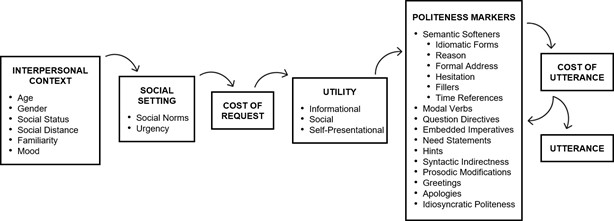
\includegraphics{C:/Users/Hannah/Desktop/preferring_politeness/figures/diagrams/contextual_considerations.jpg}
\caption{Considerations when selecting a polite utterance.}
\end{figure}

\newpage

In selecting a polite utterance, an individual must first consider the interpersonal context of their interaction. According to Lakoff's (1973) first rule of politeness (\emph{Distance}), it is important for speakers to avoid imposing by maintaining the social distance between themselves and their interlocutors. To be appropriately polite, an individual must vary their level and form of linguistic politeness depending on this social distance, which may be evinced in age, gender, occupation, and social status (Lakoff, 1973; Pedlow, Wales, \& Sanson, 2001). For example, it may be more appropriate for a younger person to speak more politely to an older person than to someone of a similar age, and it may be more appropriate for a male to speak more politely to a female than to another male.

After considering the interpersonal context of their interaction, a person must consider the degree of politeness which is appropriate for the unique social setting. For instance, a sense of urgency makes it more appropriate to opt for the imperative (and less polite) phrase ``Call an ambulance, now,'' as opposed to asking, ``Ms.~Smith, when you have a moment, would you mind calling an ambulance, please?''

After considering the interpersonal context and social setting of their interaction, an appropriately polite individual must consider the cost of their request and, if applicable, redress an overly costly request by increasing their degree of linguistic politeness (Labov \& Fanshel, 1977).

Based on the utility-theoretic explanation of politeness goals, an individual must also decide how informative they want to be, how kind they want to be, and how informative and kind they want to appear. In doing so, the person must determine their ideal, balanced weightings of the informational, social, and self- presentational utilities of their utterance (Yoon, Tessler, Goodman, \& Frank, 2020).

Then, the individual must consult their internal inventory of politeness markers and selectively compose an utterance which is appropriate for the interpersonal context, social setting, and cost of their request, as well as satisfies their desired utilities. As formalized by Lakoff (1973), requests which are more imposing, present fewer options, and risk making the addressee feel bad require heightened polite speech.

Finally, the person must weigh the cost of their utterance (e.g., a long utterance or an utterance that compromises utility would be particularly costly). If the cost is reasonable, then the person would make the utterance, and if the utterance is too costly, the person would return to their inventory of politeness markers to compose a less costly utterance.

The broader context in which an individual composes a polite utterance can be understood through a Rational Speech Act (RSA) framework (Yoon, Tessler, Goodman, \& Frank, 2020). RSA models (Frank \& Goodman, 2012) are based on the theory that probabilistic speakers and probabilistic listeners recursively reason about each other's mental states in order to infer the intended meaning of utterances and to generate responses. At each step in the process of composing a polite utterance, the speaker must not only judge the literal meaning of their own potential utterance; they must also predict the listener's interpretation to ensure that their utterance effectively communicates their intended message.

According to this RSA framework, a speaker chooses to produce an utterance containing particular politeness markers based on their prediction of how a listener would interpret it, and the listener interprets the utterance by reasoning about the speaker's prediction, and so on (Yoon, Tessler, Goodman, \& Frank, 2020).

\hypertarget{acquisition-of-politeness}{%
\subsection{Acquisition of Politeness}\label{acquisition-of-politeness}}

Being suitably polite involves masterfully combining an understanding of social and contextual factors with an inventory of linguistic forms. The complexity of this ability brings into question when and how humans begin to acquire polite speech.

Production of polite speech begins early in development among English-speaking children: At 2 years, children modify their requests to adjust politeness (Bates \& Silvern, 1977). At 2.5 years, children produce the word ``please'' (Read \& Cherry, 1978) and use hints as an indirect request strategy (Newcombe \& Zaslow, 1981). By 3 years, children are able to vary their utterances based on whether they are instructed to ``tell'' versus ``ask'' an addressee to give them a puzzle piece (Bock \& Hornsby, 1981). 3-year-old children also possess several politeness formulas in their repertoires and use them spontaneously and appropriately quite frequently in their home context (Eisenberg, 1982).

Evidence from studies on children's understanding of politeness indicates that children understand the implications of polite speech early on. In a study by Yoon and Frank (2019), each child was read 12 stories in which two characters made requests politely and impolitely. The child was then asked one of four speaker attribute questions (``Which one was more polite/more rude/nicer/meaner{]}?'') and one of two social implication questions (either ``Which one would you rather play with?'' or ``Which one will {[}get what they want{]}?''). Yoon and Frank ran three experiments which tested different combinations of linguistic markers, prosodic cues, and facial expressions. They observed no substantial effect of prosodic cues or facial expression; children's inferences seemed to be supported solely by linguistic markers. They found that by 3 years, preschool children could correctly identify whether a person was more polite, more rude, nicer, or meaner than another speaker based on which speaker included politeness markers like ``please'' in their requests. By 4 years, preschool children understood that polite speakers are more likely to have their requests granted and tended to choose polite speakers as play partners over non-polite speakers; however, this study did not observe reliable preference for a polite speaker in children younger than 4 years.

Because (1) children tend to comprehend language before producing it (Clark \& Hecht, 1983), (2) children produce ``please'' at 2.5 years (Read \& Cherry, 1978), (3) polite language is considered prosocial (Brown \& Levinson, 1978), and (4) infants as young as 6 months prefer prosocial characters (Hamlin, Wynn, \& Bloom, 2007), it seems plausible that children at least as young as 2.5 years should indicate preference for a polite speaker. Considering this, Yoon and Frank may have not observed reliable preference for a polite speaker in children younger than 4 years due to experimental task demands.

The stimuli used by Yoon and Frank was visually complex with detailed characters and backgrounds, which may have distracted children from the characters' speech. Because the children were read a series of 12 stories, performance on the task required a long attention span. Further, the stories were narrated, so the superfluous auditory input may have made it difficult for younger children to note the difference between polite and impolite speech. Overall, these features of the stimuli may have made the task less accessible to younger children.

\begin{figure}
\centering
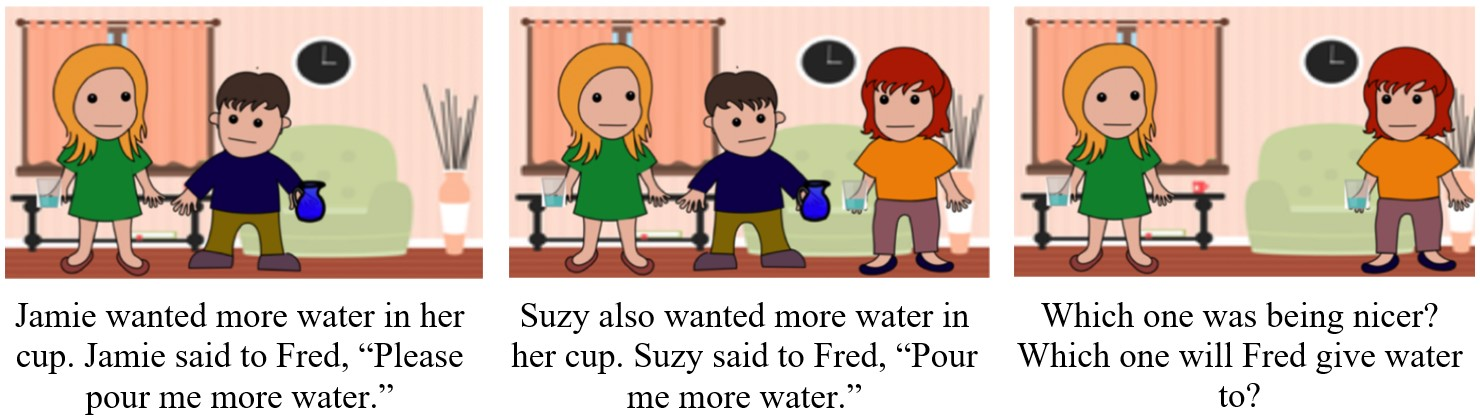
\includegraphics{C:/Users/Hannah/Desktop/preferring_politeness/figures/images/yoon2019.jpg}
\caption{Stimuli sample from Yoon and Frank (2019).}
\end{figure}

There is a precedent of using shape-preference paradigms when assessing social preference in very young children. Both Hamlin et al.~(2007) and Thomas and Sarnecka (2019) employ shape-preference paradigms in which characters are represented by colored shapes with eyes and a mouth to indicate animacy. This type of paradigm may be more accessible to young children than more visually complex stimuli; basic colors and shapes allow children to easily distinguish between the characters without visual distraction.

\newpage

\begin{figure}
\centering
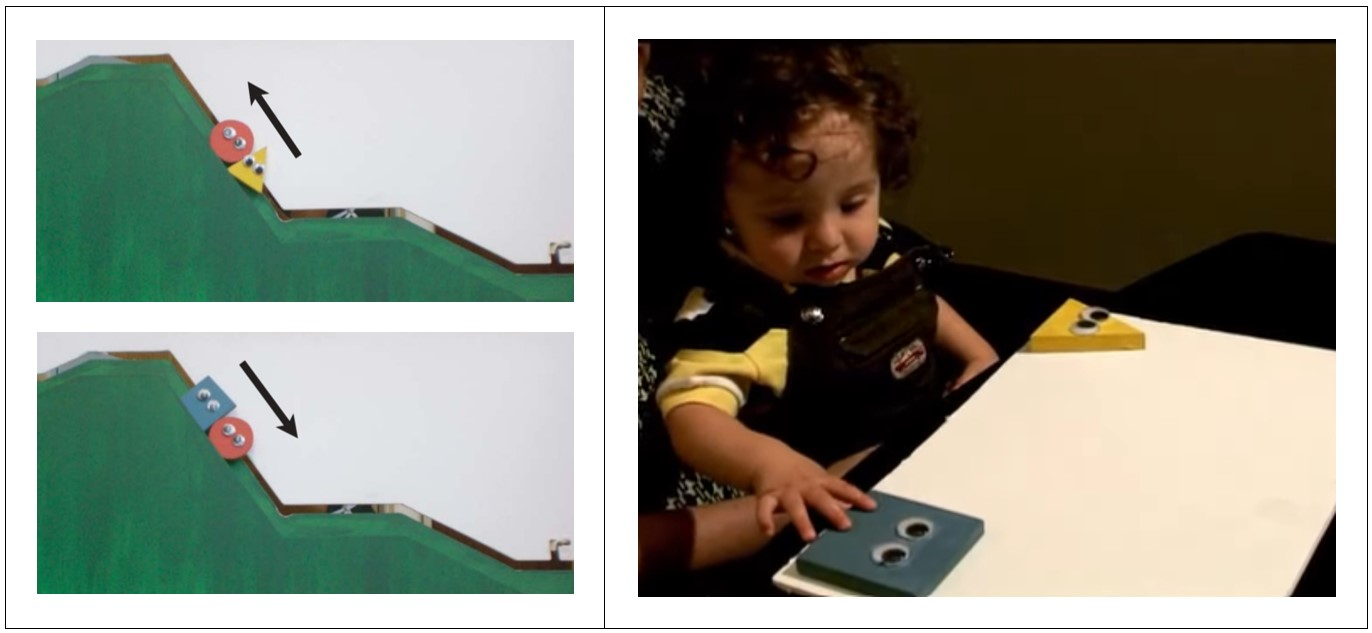
\includegraphics{C:/Users/Hannah/Desktop/preferring_politeness/figures/images/hamlin2007.jpg}
\caption{Stimuli sample from Hamlin et al.~(2007). A character attempted to climb a hill and was either bumped up the hill by a helper (top left panel) or bumped down the hill by a hinderer (bottom left panel). The child was presented with the helper and hinder (right panel), and the child's grabbing or reaching behavior was treated as indication of preference.}
\end{figure}

\newpage

\begin{figure}
\centering
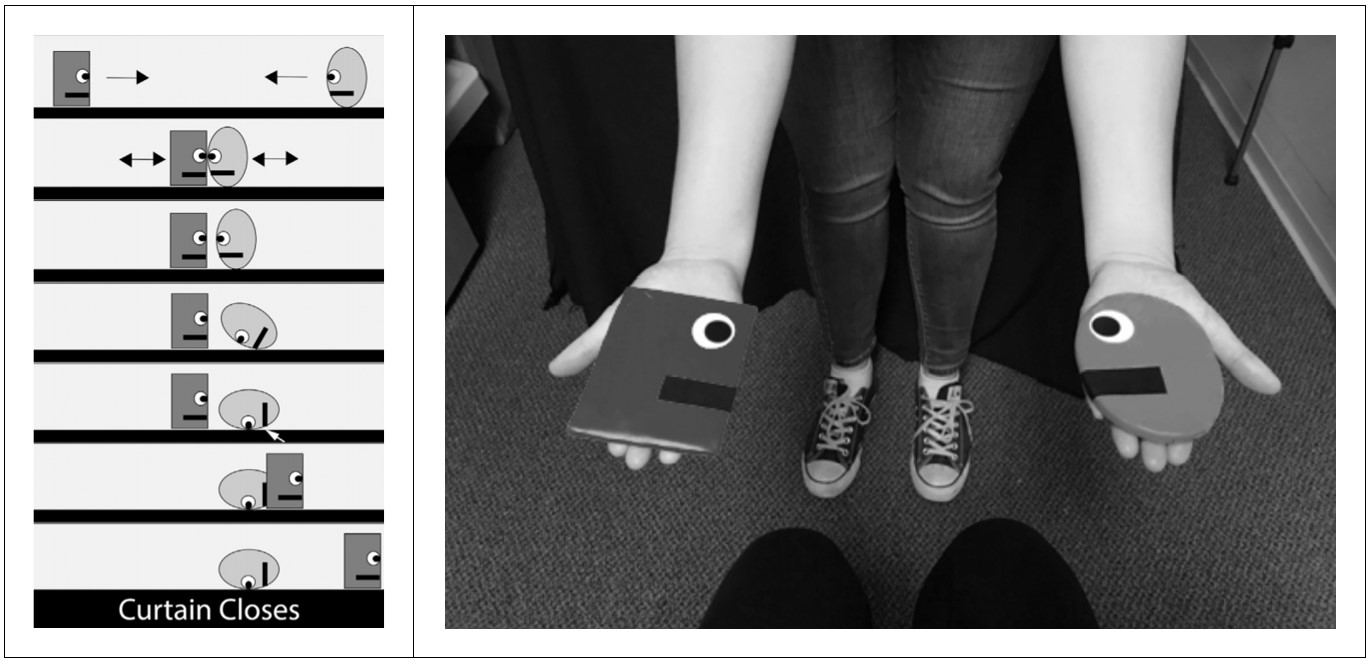
\includegraphics{C:/Users/Hannah/Desktop/preferring_politeness/figures/images/thomas2019.jpg}
\caption{Stimuli sample from Thomas and Sarnecka (2019). A high-status and a low-status character approached each other and collided. The low-status character yielded by bowing and moving upstage (left panel). The child was presented with the high-status and low-status puppets (right panel), and the child's grabbing or reaching behavior was treated as indication of preference.}
\end{figure}

\newpage

\hypertarget{the-current-study}{%
\subsection{The Current Study}\label{the-current-study}}

The current study tests 2-year-old, 3-year-old, and 4-year-old children's implicit understanding of linguistic politeness by assessing their preference for a polite speaker over an impolite speaker.

In this study, we adopt a visually simple shape-preference paradigm (Hamlin, Wynn, \& Bloom, 2007; Thomas \& Sarnecka, 2019) to minimize visual distractions and to assist children in distinguishing between characters more easily. Our stimuli consist of only two animations--one featuring a polite speaker and one featuring an impolite speaker--so children do not have to pay attention for very long. To minimize auditory distractions, our stimuli involve no narration: The only audible speech is the polite and impolite utterances.

By making these adjustments, the current study proposes a more accessible task, which could detect preference for a polite speaker in children younger than 4 years.

\hypertarget{hypotheses}{%
\subsubsection{Hypotheses}\label{hypotheses}}

\begin{enumerate}
\def\labelenumi{\arabic{enumi}.}
\item
  Considering our less challenging task, we predicted that 2-year-old, 3-year-old, and 4-year-old children would indicate preference for a polite speaker over an impolite speaker (i.e., the proportion of children in each age category who indicated preference for a polite speaker would differ from chance).
\item
  Considering evidence for graded comprehension of politeness in young children (Yoon \& Frank, 2019), we predicted that children would indicate preference for a polite speaker over an impolite speaker more reliably with increasing age.
\end{enumerate}

\newpage

\hypertarget{methods}{%
\section{Methods}\label{methods}}

\hypertarget{participants}{%
\subsection{Participants}\label{participants}}

Participants (\emph{N} = 56; 15 Asian, 1 Black/African, 1 Hispanic/Latinx, 1 Native American, 29 White, 6 more than one race, 3 unreported race) included English-speaking 2-year-old (\emph{n} = 18; 9 male, \(M_{age}\) = 2.52 years, \(SD_{age}\) = 0.23), 3-year-old (\emph{n} = 18; 7 male, \(M_{age}\) = 3.58 years, \(SD_{age}\) = 0.32) and 4-year-old children (\emph{n} = 20; 10 male, \(M_{age}\) = 4.55 years, \(SD_{age}\) = 0.31) children living in the U.S.A. at the time of data collection. Participants were recruited through the Department of Psychology at Stanford University through Facebook advertisements, Children Helping Science (an online recruitment platform for developmental research), and direct outreach to preschools and day cares in the Bay Area.

We selected our sample size based on a Bayesian power analysis conducted in R. Our lowest-power statistical tests were by-age-category Bayesian binomial tests. To detect an effect in which 80\% of children indicate preference for a polite speaker with 80\% power and a 95\% credible interval, we ran 15 participants in each age category (45 total). We recruited 60 participants to compensate for exclusions and missing data. A second power analysis showed that with 60 participants across age categories, we could detect an effect in which 70\% of children indicate preference for a polite speaker with 80\% power and a 95\% credible interval.

Prior to data collection, we decided to exclude a child from the study if:

\begin{enumerate}
\def\labelenumi{\arabic{enumi}.}
\item
  The child was known to have any cognitive, auditory, or visual impairment, and the impairment was reported by the parent.
\item
  The child was known to have any neurodevelopmental disorder that significantly affects cognitive processing or social cognition, such as Down syndrome or autism spectrum disorder, and the disorder was reported by the parent. Attention deficit disorder and attention deficit hyperactivity disorder were only grounds for exclusion if the child was unable to adequately complete test trials due to inattention or restlessness as per criterion 6.
\item
  The child did not hear English ``all of the time'' or ``most of the time'' as indicated by the parent upon registration.
\item
  A non-participant (e.g., the child's parent or sibling) interjected or interfered by pointing at the screen at any time during the experiment, audibly commenting, or providing a response to either dependent variable measure.
\item
  The child failed to provide a response to DV1 after four prompts.
\item
  The child was looking away from the screen for at least 25\% of the animation.
\item
  The child was looking away from the screen during either speaker utterance.
\item
  The parent rated the video or audio quality below a 3 out of 5.
\end{enumerate}

\hypertarget{stimuli}{%
\subsection{Stimuli}\label{stimuli}}

The animation began with a secondary familiarization phase (Figure 5) in which a shape (the speaker) entered from the left of the screen, spotted two cookies on the opposite side of the screen, gasped excitedly, approached the cookies, ate one cookie, and celebrated by jumping up and down. The purpose of this phase was to inform the participant that the speaker's goal was to eat a cookie.

\begin{figure}
\centering
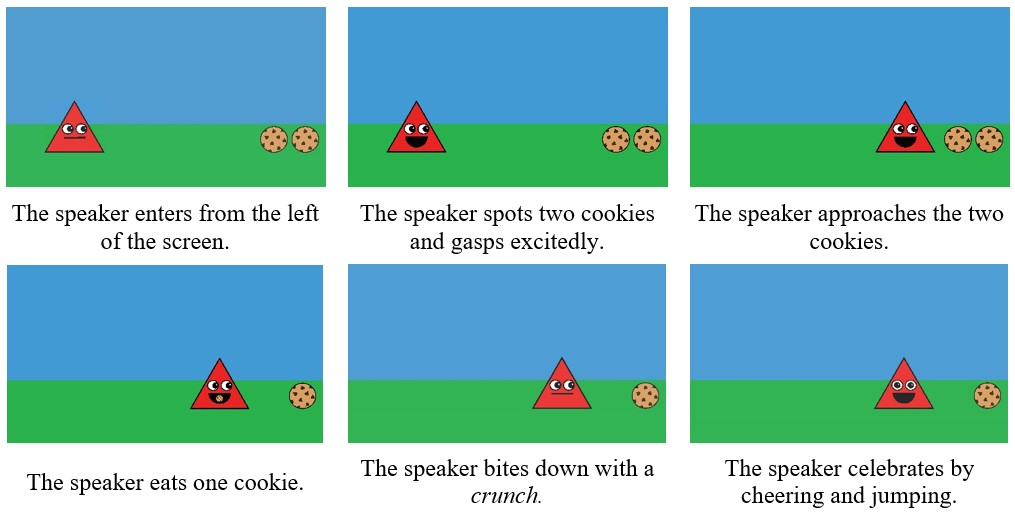
\includegraphics{C:/Users/Hannah/Desktop/preferring_politeness/figures/images/familiarization.jpg}
\caption{Familiarization phase.}
\end{figure}

A testing phase (Figure 6) followed in which the speaker entered from the left of the screen and stopped in front of another shape (the listener), who was standing in the way of the cookies. In the polite condition, the speaker said, ``I am so hungry! May I have a cookie, please?'' In the impolite condition, the speaker said, ``I am so hungry! Give me a cookie now.'' Regardless of condition, the listener moved out of the speaker's way. The speaker gasped excitedly, crossed in front of the listener, approached the cookies, ate one cookie, and celebrated by jumping up and down.

\begin{figure}
\centering
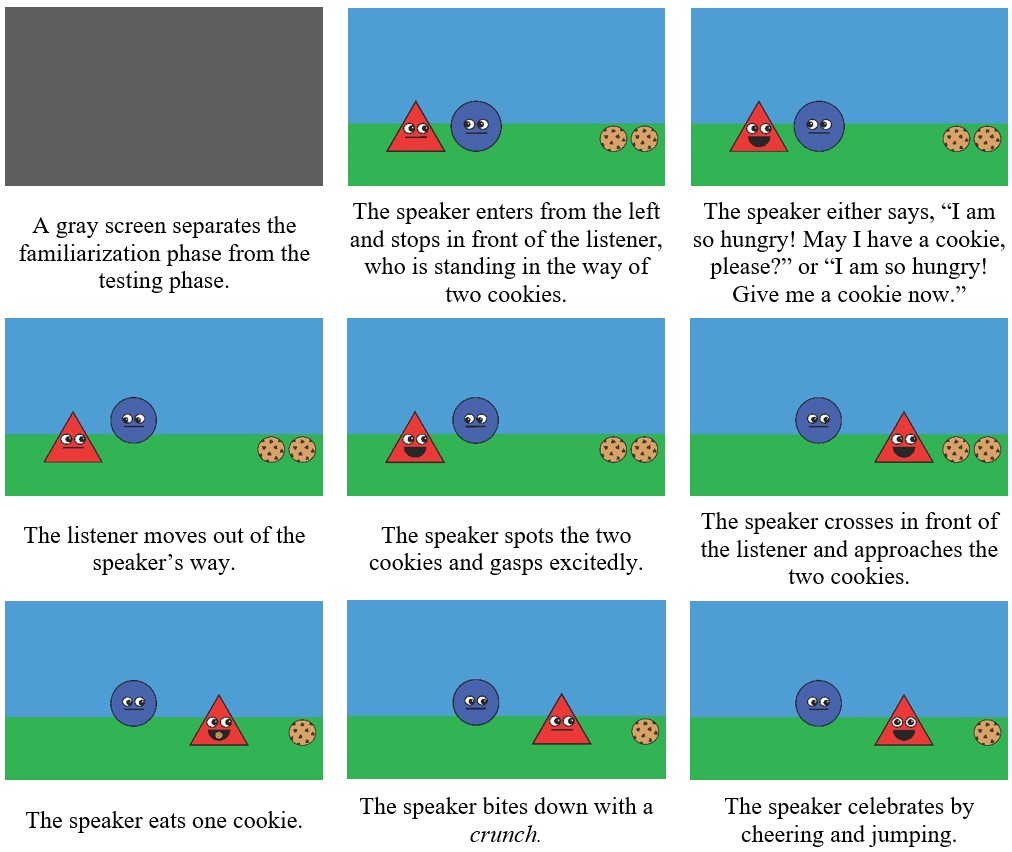
\includegraphics{C:/Users/Hannah/Desktop/preferring_politeness/figures/images/testing.jpg}
\caption{Testing phase.}
\end{figure}

Utterances used in the animation were prerecorded. To ensure children would make inferences based on linguistic markers alone, intonation was naturalistic and did not include exaggerated ``polite'' or ``impolite'' prosody. Utterances were cleaned using Audacity, an audio editing and recording software (Audacity Team, 2020), and RMS was standardized across conditions using Praat, a phonetics software (Boersman \& Weenink, 2020).

The background consisted of a solid, green block and solid, blue block depicting grass and sky. The listener was always a blue circle. The polite and impolite speakers were represented by either a red triangle and yellow square, respectively, or a yellow triangle and red square, respectively. The triangle and square were the same height and width. The shape of the speaker (triangle/square), color of the shape (red/yellow), and order of the conditions (first/second) were counterbalanced across trials.

\hypertarget{randomization}{%
\subsection{Randomization}\label{randomization}}

A generic list randomizer was used to assign the first 16 participants in each age category to one of 16 uniquely counterbalanced animations (without repeats). The same generic list randomizer was used to assign the remaining four participants in each age category to one of the 16 animations (without repeats).

\hypertarget{procedure}{%
\subsection{Procedure}\label{procedure}}

Children completed the study in their family's home on personal computers with an experimenter online via Zoom (a videotelephony software). A parent provided either written consent via email or verbal consent prior to testing. The attending parent was notified that they or their child may stop participation at any time. Testing sessions were recorded with parental consent. Each session began by testing audio quality and calibrating the participant's screen settings.

The experimenter began with a warm-up activity to build rapport with the child. The experimenter played a short I-Spy game with the child, during which a black and white dog emerged from behind a pile of leaves, then a brown squirrel emerged from the same pile. To avoid inducing side bias, the animals were front-facing and centered, and the pile of leaves was symmetrical.

Next, in the primary familiarization, the experimenter introduced the child to a green pentagon, which had eyes and a mouth to indicate animacy. The experimenter then showed the child what the character looks like when it ``feels very sad'' (downturned mouth), ``feels normal'' (flat-line mouth), and ``feels very happy'' (upturned, open mouth). The purpose of this primary phase was to introduce shapes as animate characters and to accustom the participant to facial expressions that would be seen in the upcoming animation.

After the primary familiarization phase, the animation was played. Each participant saw both the polite condition and the impolite condition as detailed above. The experimenter was not blind to condition but bared a blank expression and looked down while the animation was playing. At the end of the animation, the caregiver attending to the child was asked to close their eyes before the child's preference and reasoning were assessed.

We measured preference between a polite speaker and an impolite speaker by presenting a forced-choice in which the speakers appeared on opposite sides of the screen (counterbalanced), and the participant was asked, ``Which friend do you want to play with?'' (DV1, our key dependent variable measure).

Pointing, reaching, and verbal answers were coded equivalently as indication of preference. If a child did not answer, the child was prompted three more times with analogous wording. If the child did not provide an answer after four prompts, the session was concluded. If the child provided an answer, the child was then asked, ``Why do you want to play with that friend?'' (DV2, a supplementary dependent variable measure). If the child did not provide an answer, the child was prompted twice more before the experiment was concluded.

Including screen setup and debriefing, each session took approximately 10 to 15 minutes to complete. Following the session, parents were emailed a certificate of participation for their child; children nor parents were financially compensated.

\hypertarget{coding-and-inferences}{%
\subsection{Coding and Inferences}\label{coding-and-inferences}}

Age category was coded to consist of three levels:

\begin{itemize}
\item
  2-year-old children (2 years, 0 months \(\leqslant\) x \textless{} 3 years, 0 months)
\item
  3-year-old children (3 years, 0 months \(\leqslant\) x \textless{} 4 years, 0 months)
\item
  4-year-old children (4 years, 0 months \(\leqslant\) x \textless{} 5 years, 0 months)
\end{itemize}

DV1 was dummy coded with preference for the polite speaker as 1 and preference for the impolite speaker as 0. DV2 was coded to include:

\begin{itemize}
\item
  No reasoning: no explanation after a third prompt (e.g., silence, shrugging, or ``I don't know'').
\item
  Superficial reasoning: any explanation regarding elements besides speaker utterance (e.g., ``I like him,'' ``He's red,'' or ``Triangles are my favorite'').
\item
  Logical reasoning: any explanation that refers to speaker utterance and is consistent with the animation (e.g., describing the polite speaker as ``nice'' or ``polite'').
\item
  Other reasoning: any explanation or utterance that cannot be classified by the three other reasoning types (e.g., an intelligible response).
\end{itemize}

Our study used pairwise deletion: If a child did not complete DV2, their DV1 data was still included in analyses. Two-tailed tests were used for each of our analyses. We made inferences based on credible intervals, using a 95\% credible interval criterion for success.

\hypertarget{results}{%
\section{Results}\label{results}}

We assessed whether the proportion of children in our sample who indicated preference for a polite speaker differed from chance using a Bayesian binomial test. 57\% of our entire sample indicated preference for a polite speaker. The probability that 2-year-old, 3-year-old, and 4-year-old children indicate preference for a polite speaker above chance level is 0.859.

A logistic regression predicting speaker preference from age indicated that at 24 months, children should indicate preference for a polite speaker over an impolite speaker with aprobability of 0.5: at chance. The model showed a slightly positive--but not particularly strong--overall effect of age: Every 12-month increase in age predicted an increase of 0.1 in the probability that a child would indicate preference for a polite speaker (see Figure 7).

To ensure we were able to characterize any variation that was not captured by our logistic regression, we faceted our data by age category. We then assessed whether the proportion of children in each age category who indicated preference for a polite speaker differed from chance, once again using Bayesian binomial tests.

66\% of 2-year-old children indicated preference for a polite speaker. The probability that 2-year-old children indicate preference for a polite speaker \emph{above} chance level is 0.920. 34\% of 3-year-old children indicated preference for a polite speaker. The probability that 3-year-old children indicate preference for a polite speaker \emph{below} chance level is 0.914. 69\% of 4-year-old children indicated preference for a polite speaker. The probability that 4-year-old children indicate preference for a polite speaker \emph{above} chance level is 0.959.

\begin{figure}
\centering
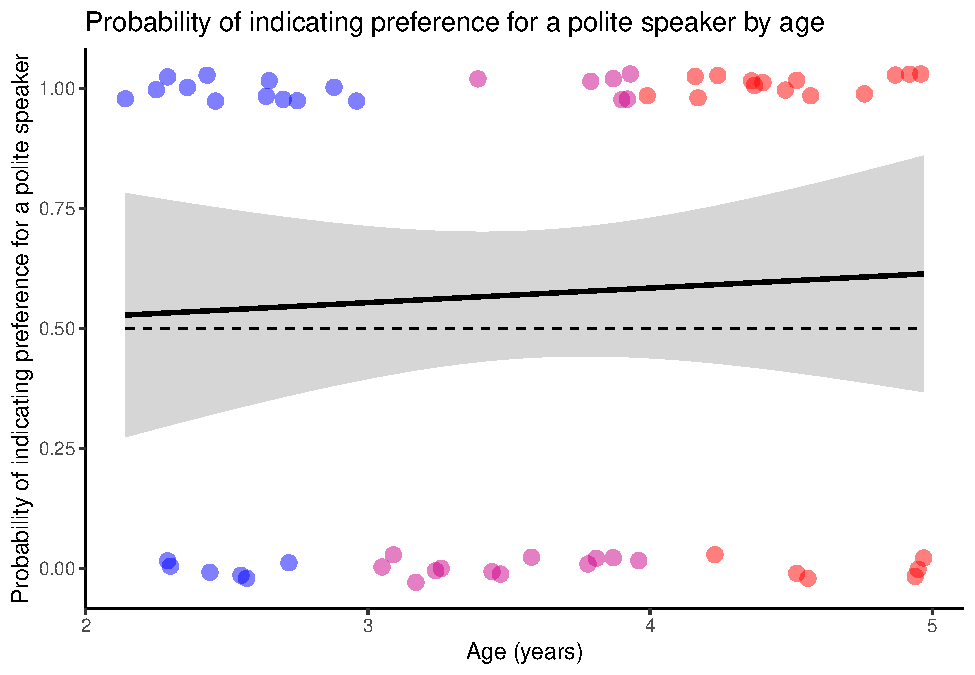
\includegraphics{writeup_files/figure-latex/unnamed-chunk-1-1.pdf}
\caption{\label{fig:unnamed-chunk-1}Each point represents an individual observation. Points have been jittered vertically for readability. Dotted, black line denotes chance performance. Solid, black line represents a logistic regression. Ribbons represent pointwise 95\% confidence intervals on the model.}
\end{figure}

\begin{figure}
\centering
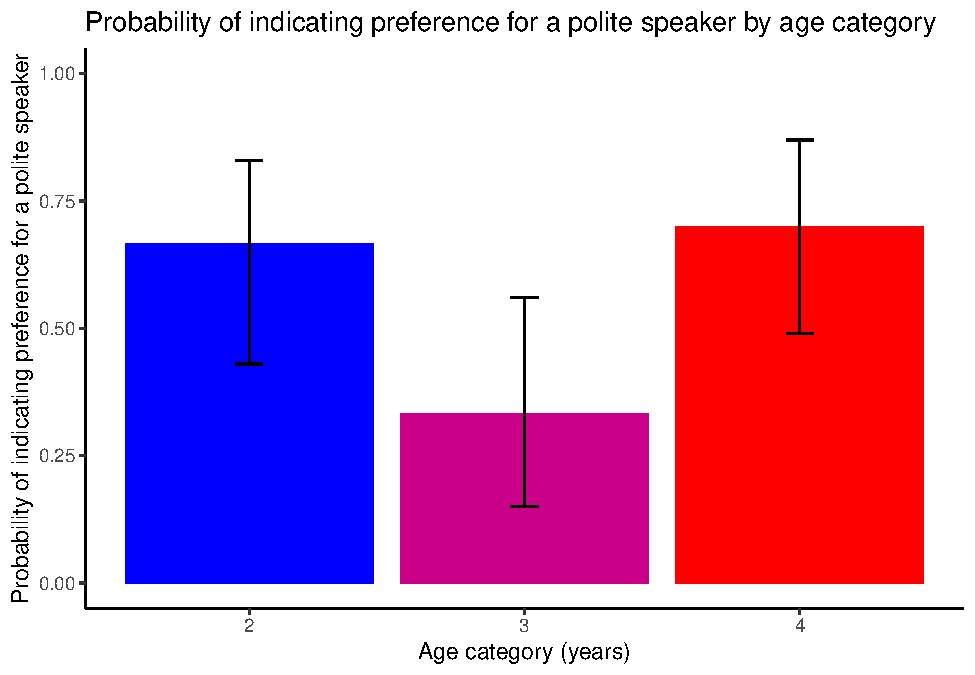
\includegraphics{writeup_files/figure-latex/unnamed-chunk-2-1.pdf}
\caption{\label{fig:unnamed-chunk-2}Each bar illustrates the mean response of participants in each age category, which is representative of the probability of indicating preference for a polite speaker. Error bars represent 95\% credible intervals based on Bayesian binomial tests.}
\end{figure}

\newpage

\begin{verbatim}
## # A tibble: 8 x 3
## # Groups:   age_category [3]
##   age_category reasoning       n
##          <int> <chr>       <int>
## 1            2 none            9
## 2            2 other           3
## 3            2 superficial     6
## 4            3 none            5
## 5            3 superficial    13
## 6            4 logical         3
## 7            4 none            4
## 8            4 superficial    13
\end{verbatim}

\hypertarget{exploratory-analyses}{%
\section{Exploratory Analyses}\label{exploratory-analyses}}

Our supplementary dependent variable measure did not elicit consequential responses. We observed a slight increase in more advanced reasoning with age: Among 2-year-old subjects, 0\% provided logical reasoning, 33\% provided superficial reasoning, 44\% provided no reasoning, and 22\% provided other reasoning. Among 3-year-old subjects, 0\% provided logical reasoning, 72\% provided superficial reasoning, and 28\% provided no reasoning. Among 4-year-old subjects, 15\% provided logical reasoning, 65\% provided superficial reasoning, and 20\% provided no reasoning. Anecdotally, these data might indicate that comprehension of linguistic politeness begins as implicit and becomes more explicit with age; however, assessing explicit comprehension is difficult in developmental psychology because young children's linguistic capabilities may prevent them from communicating an internal, explicit understanding.

\begin{verbatim}
## Warning: Problem with `mutate()` input `reasoning`.
## i Unknown levels in `f`: logical
## i Input `reasoning` is `fct_relevel(reasoning, "other", "none", "superficial", "logical")`.
## i The error occurred in group 1: age_category = 2.
\end{verbatim}

\begin{verbatim}
## Warning: Problem with `mutate()` input `reasoning`.
## i Unknown levels in `f`: other, logical
## i Input `reasoning` is `fct_relevel(reasoning, "other", "none", "superficial", "logical")`.
## i The error occurred in group 2: age_category = 3.
\end{verbatim}

\begin{verbatim}
## Warning: Problem with `mutate()` input `reasoning`.
## i Unknown levels in `f`: other
## i Input `reasoning` is `fct_relevel(reasoning, "other", "none", "superficial", "logical")`.
## i The error occurred in group 3: age_category = 4.
\end{verbatim}

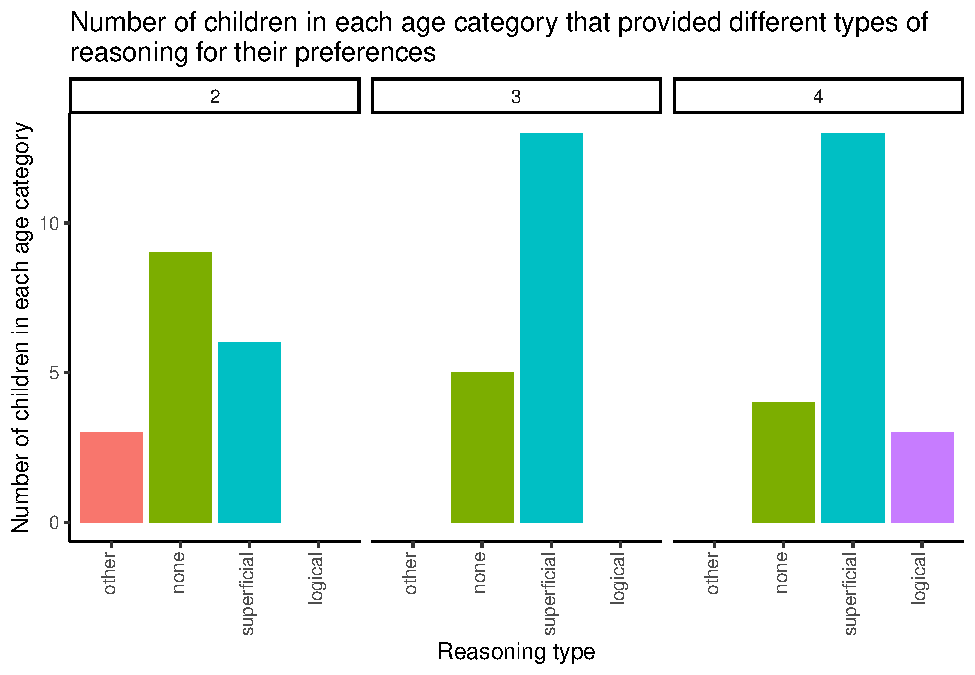
\includegraphics{writeup_files/figure-latex/unnamed-chunk-3-1.pdf}

\hypertarget{discussion}{%
\section{Discussion}\label{discussion}}

In this study, we sought to determine whether children younger than 4 years possess a preference for a polite speaker over an impolite speaker. We replicated prior research which suggested that 4-year-old children reliably indicate preference for a polite speaker, whereas 3-year-old children do not (Yoon \& Frank, 2019); however, our data suggest that this is not indicative of the onset of this preference. By employing a shape-preference paradigm with fewer experimental task demands than in prior studies, we were able to show that 2-year-old children also reliably indicate preference for a polite speaker over an impolite speaker. These findings suggest that the onset of an implicit comprehension of linguistic politeness may occur as early as 2 years.

Consistent with existing literature, our study confirmed that 4-year-old children reliably indicate preference for a polite speaker (Yoon \& Frank, 2019).

In contrast to prior literature, our combined sample of 2-year-old, 3-year-old, and 4-year-old children indicated preference for a polite speaker above chance level. Our logistic regression revealed a slightly positive overall effect of age on the probability that a child would indicate preference for a polite speaker (see Figure 7). Our results offer evidence in support of our second hypothesis: Considering evidence for graded comprehension of politeness in young children (Yoon \& Frank, 2019), we predicted that children would indicate preference for a polite speaker over an impolite speaker more reliably with increasing age.

Further, the intercept of our model revealed performance above chance as early as 2 years. This finding suggests that socio-pragmatic competence--specifically implicit comprehension of linguistic politeness as indicated by preference for a polite speaker--is established as early as 2 years: 2 years earlier than alleged by prior research.

The performance of 2-year-old children in our task is comparable to the performance of 4-year-old children, indicating that there is not a substantial increase in the probability of indicating preference for a polite speaker between 2 and 4 years: All of the cognitive capacities that are necessary for identifying politeness markers, forming an opinion about the speaker based on these markers, and indicating a preference is present at 2 years.

There is strong evidence that infants as young as 6 months are capable of social evaluation and prefer prosocial others to antisocial others (Hamlin, Wynn, \& Bloom, 2007). Children begin producing polite language as early as 2 years (Bates \& Silvern, 1977; Read \& Cherry, 1978), and children understand language prior to producing it. Reconciling this existing literature with our data suggests that by 2 years, children recognize polite language as prosocial, which motivates them to prefer polite speakers over impolite speakers. This understanding of polite language as an indicator of prosociality may be due in part to children recognizing the co-occurrence of politeness markers and other positive words, for example, ``You should be nice and say please'' (Yoon \& Frank, 2019).

As an alternative to this preference for prosocial language, children may prefer polite speakers due to the reinforcement they receive from adults early on in development. English-speaking children are often explicitly taught and prompted to use politeness markers in their requests from early on (Gleason \& Weintraub, 1976). Adults often praise polite language and good manners in children. Further, adults are more likely to grant the requests of children who speak politely.

Our sample of 3-year-old children performed much differently than expected: 3-year-old children performed \emph{below} chance, indicating preference for the impolite speaker. While we observed a numerical dip in the probability of 3-year-old children indicating preference for a polite speaker, our intuition is that this is not indicative of a true declivity. It is unusual for developmental trajectories to be characterized by a temporary slump; therefore, our data may under-estimate the true probability of 3-year-old children indicating preference for a polite speaker. Unfortunately, our sample size was not large enough to assuredly discern the difference between a chance deviation and a true deviation from our hypothesized developmental trajectory. In order to make this distinction, our results will have to be replicated.

It is, however, possible that the numerical dip we observed in 3-year-old children is indicative of a true developmental trend. If replicated, this finding would be meaningful because it would demonstrate that, contrary to prior belief, preference for a polite speaker--and perhaps comprehension and acquisition of linguistic politeness more broadly--does not develop as a smooth, upward trend across development.

At 3 years, most children enter preschool, at which point they experience a sudden increase in their social interaction with peers. In this socially rich environment, children may be more interested in \emph{exploring} the social world and thus select the character whose utterance is the least expected as opposed to the character whose utterance is the most prosocial. By 4 years, children have gained significant experience with the social world and consequences of prosocial and antisocial behavior, which may cause them to revert back to preferring prosocial others.

While preference for a polite speaker, itself, is a meaningful measure of socio-pragmatic competence, preference for a polite speaker may not sufficiently capture children's implicit comprehension of linguistic politeness. In this study, we use preference for a polite speaker as an operationalization of implicit comprehension of linguistic politeness; however, this measurement masks comprehension of linguistic politeness that manifests as preference for an impolite speaker.

Some children may prefer an impolite speaker due to the unexpected nature of the speaker's language. There is compelling evidence that young children prefer--and choose to engage with--toys which function unexpectedly (Bonawitz, Schijndel, Friel, \& Schulz, 2012; Gweon \& Schulz, 2008; Schulz \& Bonawitz, 2007). The context that is presented in our animation is foreign to many children: From a very young age, if a child asks nicely, their wishes are granted, and if they ask rudely, they are corrected by an adult (e.g., ``What do you say?'' or ``What's the magic word?''). In our animation, the request of both the polite and impolite characters were granted. The unexpected response to the impolite speaker may motivate some children to prefer the impolite speaker.

It is also worth noting that multiple children in our sample distinctly giggled after the impolite speaker made its utterance. In response to DV2, some children even credited their choice of the impolite speaker to their perception of the speaker as ``funny'' or ``silly.'' Humor, as a component of social interaction, may contribute to some children's interest in and preference for impolite speakers.

Politeness is extremely broad and is used across several contexts (see Figure 1). As such, this study was only able to examine children's preference for a polite speaker in a very specific scenario, one which represents only a very small portion of the landscape in which linguistic politeness is usually employed. Children's preference for a polite speaker may vary across contexts. Likewise, there is myriad evidence that children hone their contextual use of politeness as they age (Axia \& Baroni, 1985; Bates \& Silvern, 1977; Becker \& Smenner, 1986; Ervin-Tripp, 1977; Gleason \& Weintraub, 1976; James, 1978; Wood, 1980); thus, young children may only possess preference for a polite speaker or, more broadly, comprehension of linguistic politeness in a limited number of social contexts.

Through this study, we developed and demonstrated the effectiveness of a more accessible paradigm for studying politeness in young children. We discovered that children younger that 4 years are able to reliably indicate preference for a polite speaker; however, we unexpectedly observed a dip in the developmental trajectory of this preference, as seen in 3-year-old children. This dip may be an artifact of the paradigm, a chance result, or indicative of a true change in preference. In order to confirm our findings, they must be replicated. Once replicated, our shape-preference paradigm can be used to study other aspects of linguistic politeness and further untangle the question of how to characterize young children's acquisition and conceptualization of polite language.

\hypertarget{supplementary-materials}{%
\section{Supplementary Materials}\label{supplementary-materials}}

\hypertarget{pre-registration}{%
\subsection{Pre-Registration}\label{pre-registration}}

The current study, including all analyses, was registered on OSF prior to data collection: \url{https://osf.io/dz8vp}.

\hypertarget{data-availability}{%
\subsection{Data Availability}\label{data-availability}}

All code, data, figures, cited papers, and pre-planned analyses are publicly available at \url{https://github.com/HannahEveMarshall/preferring_politeness}.

\newpage

\hypertarget{references}{%
\section{References}\label{references}}

\begingroup
\setlength{\parindent}{-0.5in}
\setlength{\leftskip}{0.5in}

\hypertarget{refs}{}
\begin{CSLReferences}{1}{0}
\leavevmode\hypertarget{ref-audacity2020}{}%
Audacity Team. (2020). {GTS}: {GNU} {Triangulated} {Surface} library. \url{https://audacityteam.org/}.

\leavevmode\hypertarget{ref-axia1985}{}%
Axia, G., \& Baroni, M. R. (1985). Linguistic politeness at different age levels. \emph{Child Development}, 918--927.

\leavevmode\hypertarget{ref-bates1977}{}%
Bates, E., \& Silvern, L. (1977). Social adjustment and politeness in preschoolers. \emph{Journal of Communication}.

\leavevmode\hypertarget{ref-becker1986}{}%
Becker, J. A., \& Smenner, P. C. (1986). The spontaneous use of thank you by preschoolers as a function of sex, socioeconomic status, and listener status. \emph{Language in Society}, 537--545.

\leavevmode\hypertarget{ref-bock1981}{}%
Bock, J. K., \& Hornsby, M. E. (1981). The development of directives: How children ask and tell. \emph{Journal of Child Language}, \emph{8}(1), 151--163.

\leavevmode\hypertarget{ref-boersman2020}{}%
Boersman, P., \& Weenink, D. (2020). {GTS}: {GNU} {Triangulated} {Surface} library. \url{http://www.praat.org/}.

\leavevmode\hypertarget{ref-bonawitz2012}{}%
Bonawitz, E. B., Schijndel, T. J. van, Friel, D., \& Schulz, L. (2012). Children balance theories and evidence in exploration, explanation, and learning. \emph{Cognitive Psychology}, \emph{64}(4), 215--234.

\leavevmode\hypertarget{ref-brown1978}{}%
Brown, P., \& Levinson, S. C. (1978). Universals in language usage: Politeness phenomena. In \emph{Questions and politeness: Strategies in social interaction} (pp. 56--311). Cambridge University Press.

\leavevmode\hypertarget{ref-clark1983}{}%
Clark, E. V., \& Hecht, B. F. (1983). Comprehension, production, and language acquisition. \emph{Annual Review of Psychology}, \emph{34}(1), 325--349.

\leavevmode\hypertarget{ref-eisenberg1982}{}%
Eisenberg, A. R. (1982). Understanding components of a situation: Spontaneous use of politeness routines by mexicano 2-year-olds.

\leavevmode\hypertarget{ref-ervintripp1977}{}%
Ervin-Tripp, S. (1977). Wait for me, roller skate! In \emph{Child discourse} (pp. 165--188). Elsevier.

\leavevmode\hypertarget{ref-frank2012}{}%
Frank, M. C., \& Goodman, N. D. (2012). Predicting pragmatic reasoning in language games. \emph{Science}, \emph{336}(6084), 998--998.

\leavevmode\hypertarget{ref-gleason1976}{}%
Gleason, J. B., \& Weintraub, S. (1976). The acquisition of routines in child language. \emph{Language in Society}, 129--136.

\leavevmode\hypertarget{ref-grice1975}{}%
Grice, H. P. (1975). Logic and conversation. In \emph{Speech acts} (pp. 41--58). Brill.

\leavevmode\hypertarget{ref-gweon2008}{}%
Gweon, H., \& Schulz, L. (2008). Stretching to learn: Ambiguous evidence and variability in preschoolers' exploratory play. In \emph{Proceedings of the 30th annual meeting of the cognitive science society} (pp. 570--574).

\leavevmode\hypertarget{ref-haidt2004}{}%
Haidt, J., \& Joseph, C. (2004). Intuitive ethics: How innately prepared intuitions generate culturally variable virtues. \emph{Daedalus}, \emph{133}(4), 55--66.

\leavevmode\hypertarget{ref-hamlin2007}{}%
Hamlin, J. K., Wynn, K., \& Bloom, P. (2007). Social evaluation by preverbal infants. \emph{Nature}, \emph{450}(7169), 557--559.

\leavevmode\hypertarget{ref-hauser2006}{}%
Hauser, M. (2006). \emph{Moral minds: How nature designed our universal sense of right and wrong.} Ecco/HarperCollins Publishers.

\leavevmode\hypertarget{ref-james1978}{}%
James, S. L. (1978). Effect of listener age and situation on the politeness of children's directives. \emph{Journal of Psycholinguistic Research}, \emph{7}(4), 307--317.

\leavevmode\hypertarget{ref-labov1977}{}%
Labov, W., \& Fanshel, D. (1977). \emph{Therapeutic discourse: Psychotherapy as conversation}. Academic Press.

\leavevmode\hypertarget{ref-lakoff1973}{}%
Lakoff, R. (1973). The logic of politeness; or, minding your p's and q's. In \emph{Ninth regional meeting of the chicago linguistic society} (Vol. 8, pp. 292--305). 292J305. Chicago: Chicago Linguistic Society.

\leavevmode\hypertarget{ref-newcombe1981}{}%
Newcombe, N., \& Zaslow, M. (1981). Do 2\(1/2\)-year-olds hint? A study of directive forms in the speech of 2\(1/2\)-year-old children to adults. \emph{Discourse Processes}, \emph{4}(3), 239--252.

\leavevmode\hypertarget{ref-pedlow2001}{}%
Pedlow, R., Wales, R., \& Sanson, A. (2001). Children's production and comprehension of politeness in requests: Relationships to behavioral adjustment in middle childhood. \emph{Journal of Language and Social Psychology}, \emph{20}(1-2), 23--60.

\leavevmode\hypertarget{ref-pinker2003}{}%
Pinker, S. (2003). Language as an adaptation to the cognitive niche. \emph{Studies in the Evolution of Language}, \emph{3}, 16--37.

\leavevmode\hypertarget{ref-read1978}{}%
Read, B. K., \& Cherry, L. J. (1978). Preschool children's production of directive forms. \emph{Discourse Processes}, \emph{1}(3), 233--245.

\leavevmode\hypertarget{ref-ryabova2015}{}%
Ryabova, M. (2015). Politeness strategy in everyday communication. \emph{Procedia-Social and Behavioral Sciences}, \emph{206}, 90--95.

\leavevmode\hypertarget{ref-schulz2007}{}%
Schulz, L. E., \& Bonawitz, E. B. (2007). Serious fun: Preschoolers engage in more exploratory play when evidence is confounded. \emph{Developmental Psychology}, \emph{43}(4), 1045.

\leavevmode\hypertarget{ref-thomas2019}{}%
Thomas, A. J., \& Sarnecka, B. W. (2019). Infants choose those who defer in conflicts. \emph{Current Biology}, \emph{29}(13), 2183--2189.

\leavevmode\hypertarget{ref-vergis2020}{}%
Vergis, N., \& Pell, M. D. (2020). Factors in the perception of speaker politeness: The effect of linguistic structure, imposition and prosody. \emph{Journal of Politeness Research}, \emph{16}(1), 45--84.

\leavevmode\hypertarget{ref-wood1980}{}%
Wood, B. S. (1980). How children {``get their way''};: Directives in communication. \emph{Communication Education}, \emph{29}(3), 264--272.

\leavevmode\hypertarget{ref-yoon2019}{}%
Yoon, E. J., \& Frank, M. C. (2019). Preschool children's understanding of polite requests. In \emph{CogSci} (pp. 3179--3185).

\leavevmode\hypertarget{ref-yoon2020}{}%
Yoon, E. J., Tessler, M. H., Goodman, N. D., \& Frank, M. C. (2020). Polite speech emerges from competing social goals. \emph{Open Mind}, \emph{4}, 71--87.

\end{CSLReferences}

\endgroup


\end{document}
